\documentclass[11pt,a4paper]{article}
\usepackage{amsmath}
\usepackage{amssymb}
\usepackage{graphicx}
\usepackage{verbatim}
\begin{document}
\noindent
Martin Lundfall, Henri Bunting, Malte Siemers, Patrik Bey
\begin{centering}
  \section*{Exercise sheet 11 - Machine Intelligence I}
  \end{centering}
\subsection*{11.1 - Cliques}
In the given graph, we have 10 vertices and 17 edges. These make up 10 1-vertex cliques and 17 2-vertex cliques. We also identify the 3-vertex cliques consisting of vertices\\ $\{A,C,H\},\{A, C, G\},\{B, C, D\}, \{B, C, G\}, \{C, H, I\}, \{G, H, I\}$. There is also one 4-vertex clique, among the vertices $\{C, G, H, I\}$.
\subsection*{11.2 - Cliques and Separators}
\subsection*{(a)}
The moralized graph of the DAG is an undirected graph where additional connections are added between nodes that share a child in the DAG.
\begin{figure}[h]
  \caption{Moralization of the DAG}
  \centering
  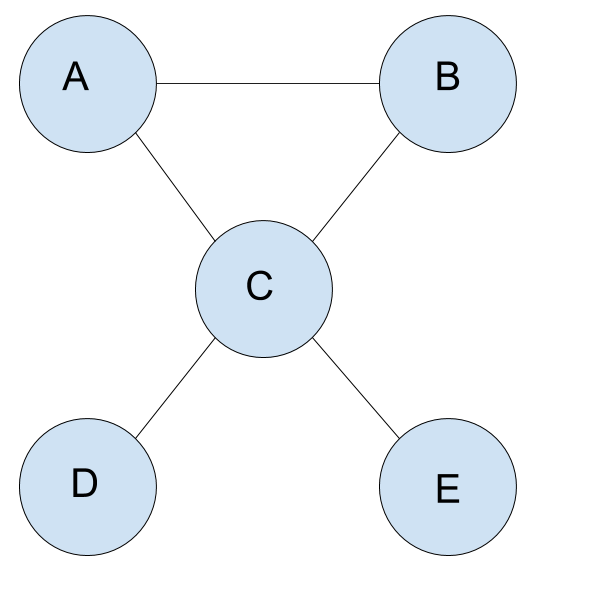
\includegraphics[width=.7\textwidth]{moral}
\end{figure}
\subsection*{(b)}
Generally, the 1-vertex cliques are all the vertices of the moral graph, the 2-vertex cliques are formed by all the vertex pairs that are directly connected, and the only 3-vertex in the graph consists of $\{A, B C\}$. The separators of the graph are $\{C\}, \{A, C\}, \{B, C\}, \{C, D\}, \{C, E\}, \{A, B, C\}, \{A, C, E\},$\\$ \{A, C, D\}, \{B, C, D\}, \{B, C, E\}$.

The given formula works only for maximal cliques and minimal separators. We have $\{A, B, C\}, \{B, C\}, \{C, E\}$ as a maximal cliques and $\{C\}$ as minimal separator.
\begin{equation}
  \begin{split}
    p(a, b, c, d, e) = p(e|c)p(d|c)p(c|a,b)p(a,b) = \\
    \\
    = \frac{p(e, c)p(d, e)p(a, b, c)p(a, b)}{p(c)p(a, b)} = \frac{p(a, b, c)p(e, c)p(d, c)}{p(c)}
    \end{split}
\end{equation}
\subsection*{11.3 Representation of the knowledge base}

\end{document}
